\section {Evaluation}
\label{sec:results}

We evaluated the effectiveness of our method on supporting juxtaposed visual comparisons and the discriminability for reading scatterplots. % by applying it to scatterplots, as scatterplots are commonly used  for such comparisons.
We conducted two online controlled experiments through Amazon Mechanical Turk (AMT) with 217 participants in total, to evaluate how well our method can support people in \emph{observing changes} and \emph{visual separability} for multiple categorical scatterplots:
\begin{enumerate}
%\vspace{-3mm}
\item [(i)] \emph{Spotting the difference task}. To evaluate how well our method can support people in \emph{observing changes} for juxtaposed categorical scatterplots;
%\vspace{-3mm}
\item [(ii)] \emph{Counting class number task}. To evaluate whether our method can support the \emph{visual separability} of classes in each individual scatterplot, which is considered fundamental to juxtaposed comparison.
%%\vspace{-3mm}
%\item [(iii)] an eye tracking study to initially explore if our method helps people \emph{alleviate eye movement distance} when performing  juxtaposed comparison tasks.
%\vspace{-3mm}
%\item [(iv)] performing two case studies to show the usability of our methods for scatterplot matrix and time series data.
\end{enumerate}
%we use synthetic data for the first three studies while use real world data for the case study.

\vspace{.3em}
\noindent{\textbf{Independent Variables.}} In each of our studies, we investigated three independent variables: colorization method, change magnitude and change type.

\emph{Colorization method}: We used six different ways to colorize scatterplots: four benchmark methods (\emph{Random Assignment}, \emph{Optimized Assignment}, \emph{Alpha Blending} and \emph{Palettailor}) and two experimental methods based on our approach (\emph{C3-Palette Assignment}, \emph{C3-Palette Generation}):
\begin{itemize}

     \item C1: \emph{Random Assignment} is randomly selecting and assigning colors from Tableau-20 palette to the classes.

     \item C2: \emph{Optimized Assignment} uses the optimized assignment approach~\cite{Wang2018} for one of the two scatterplots with an input of Tableau-20 color palette.

     \item C3: \emph{Alpha Blending} is achieved by setting the alpha of each unchanged class to $0.5$ while the changed classes remain to $1.0$ based on \emph{Optimized Assignment} result. We choose $0.5$ since the results also used in the discrimination task.
     \item C4: \emph{Palettailor} uses the method proposed by Lu et.al~\cite{Lu21} for single scatterplot palette generation. The palette is generated for one of the two scatterplots with the default settings.
     \item C5: \emph{C3-Palette Assignment} uses the color assignment optimization solution(Eq.~\ref{eq:cosaliency}) based on Tableau-20.
     \item C6: \emph{C3-Palette Generation} uses the unified color generation and assignment optimization method, and produced the results with the default parameters($\omega_0=1.0$, $\omega_1=1.0$ and $\omega_2=1.0$).
\end{itemize}
Our approach are all using the default parameters $\lambda=0.4$ and $\kappa=0$.

\emph{Change magnitude} and \emph{Change type}: While the colorization method is the primary independent variable to be investigated, we are also interested in how the effect of different methods would vary based on the level of change between the two scatterplots and the different change type of classes. Thus we first define two types of changes that a class would have across multiple scatterplots: \emph{point number} and \emph{point position}. Then for each change type, we define three levels of change magnitude calculated using Eq.~\ref{eq:cm}: \emph{small}, \emph{medium}, and \emph{large}. (See the next paragraph for the detailed calculation.)

\vspace{.3em}
\noindent{\textbf{Scatterplot Dataset Generation.}}
The paired scatterplot datasets used in our studies were generated as follows.
First, we designed a set of multi-class scatterplots, each containing $8$ classes. Each class was generated using Gaussian random sampling and placed randomly in a $600 \times 600$ area.
Similar to~\cite{Lu21}, these classes belong to one of the four settings of varying size and density: small \& dense ($n=50, \sigma=20$), small \& sparse ($n=20, \sigma=50$),  large \& dense ($n=100, \sigma=50$), and large \& sparse (($n=50, \sigma=100$).

Then, for each scatterplot generated above, we produced its paired scatterplot by randomly choosing one or more classes and changing the positions or number of their data points.
%We focused on two common change types: \emph{point number} and \emph{point position}.
To systematically compute the changes, we defined two variables: \emph{change ratio} and \emph{number of changed classes}.
\emph{Change ratio} defines how large the change of a type is, ranging from 0 to 1; and {number of changed classes} defines the number of classes that are changed, ranging from 1 to 3 (adding
different levels of difficulty). We summarize our basic idea of data generation for each change type as below.
\begin{itemize}

     \item \emph{Point number}: For each class in the original scatterplot,  we calculated the new point number by multiplying the original number by ($1 \pm$ \emph{change ratio}). An addition means to increase the point number, which was implemented by generating the new points with the same distribution as the original class. Subtraction was achieved by randomly deleting data points from the original class.

     \item \emph{Point position}: Point position contains many types, such as class center position change and shape change. In our experiment, we use the two different position changes mentioned above. For center position change, the center of a class can be moved in a certain \emph{direction} with a specific \emph{distance}. We moved the center towards a random direction by a distance calculated by multiplying a maximal change distance ($400$ by default) by the \emph{change ratio}. For shape change, we define the shape of a class as the bounding box of its data points. We simulated a shape change of a class by modifying the density parameter of its Gaussian distribution to the opposite direction. For example, a small \& dense class ($n=50, \sigma=20$) would be changed into a small \& sparse ($n=50, \sigma=50$) class. In order to produce a new shape for a class, we first calculate the one-to-one mapping between the newly-generated class and the original class using ~\cite{kuhn1955hungarian} and then linearly interpolated the new point between each two points based on the \emph{change ratio} parameter. We randomly choose one change type when disturbing the class to be changed.
\end{itemize}
For each change type, we produced 300 candidate scatterplot pairs and then calculated the \emph{change magnitude} for each pair, and split all  pairs into three levels: \emph{small},  \emph{medium}, and \emph{large}.
Next, we randomly selected $2$ pairs from each change magnitude level for each change type and each number of changed classes. Thus in total we used $36$ paired scatterplot in each of the two studies. The detailed dataset is showed in Table.~\ref{tab:latinsquare}

\begin{table}[ht]
     \renewcommand\arraystretch{1}
     \centering
     \caption{Grouping of Datasets: $36$ datasets $\times$ $6$ conditions. C: condition; G: participant group; Position Small 1: point position change with small change magnitude for 1 changed class.}
     \label{tab:latinsquare}
     \begin{tabular}{lcccccccc}
     \hline
      & C1 & C2 & C3  & C4 & C5 & C6 \\

     \hline
     Dataset 1: Position Small 1 & \textbf{G1} & G2 & G3  & G4 & G5 & G6 \\
     Dataset 2: Position Small 1 & G6 & \textbf{G1} & G2 & G3  & G4 & G5 \\
     Dataset 3: Position Small 2 & G5  & G6 & \textbf{G1} & G2 & G3 & G4 \\
     Dataset 4: Position Small 2 & G4 & G5  & G6 & \textbf{G1} & G2 & G3 \\
     Dataset 5: Position Small 3 & G3 & G4 & G5  & G6 & \textbf{G1} & G2 \\
     Dataset 6: Position Small 3 & G2 & G3 & G4  & G5 & G6 & \textbf{G1} \\
     Dataset 7: Position Medium 1 & \textbf{G1} & G2 & G3  & G4 & G5 & G6 \\
     Dataset 8: Position Medium 1 & G6 & \textbf{G1} & G2 & G3  & G4 & G5 \\
     ... & & & & & & &\\
     Dataset 35: Number Large 3 & G3 & G4 & G5  & G6 & \textbf{G1} & G2 \\
     Dataset 36: Number Large 3 & G2 & G3  & G4 & G5 & G6 & \textbf{G1}  \\

     \hline
     \end{tabular}
     \end{table}
%
%\subsection{Numeric Study}
%\label{subsec:quantitystudy}
%To evaluate whether our approach can fundamentally support the visual separability of the classes in each scatterplot, we conducted a numeric study using the \emph{class visibility metric} proposed by Kim et al.~\cite{lee2013perceptually}. We calculated each scatterplot in every pair, and used the average value as the final score of the pair. We then compared the scores across different colorization methods.
%
%%\vspace{.3em}
%%\noindent{\textbf{Results.}}
%
%\begin{figure}[h]
%\centering
%\includegraphics[width=0.9\linewidth]{figures/classVisibility.pdf}
%\caption{Average class visibility score of the 36 synthetic scatterplot pairs of each color mapping scheme.}
%\vspace*{-3mm}
%\label{fig:classVisibility}
%\end{figure}
%
%As shown in Fig.~\ref{fig:classVisibility}, \emph{Ours Generation} has the highest score on average. \emph{Ours Tableau-10} is sometimes higher than \emph{Random Tableau-10}. The two conditions based on the Tableau-20 palette have the lowest scores, and \emph{Ours Tableau-20} appears to be slightly lower than \emph{Random Tableau-20}. This might be caused by the palette used in these conditions. Since Tableau-20 consists of both saturated and de-saturated colors, \emph{Ours Tableau-20} tends to select several de-saturated colors for the classes that change less in order to make strongly changed classes more salient. Yet that might diminish the visual separability of the classes.

\subsection{Experiment 1: Spotting the Difference}
\label{subsec:onlinestudy1}

To evaluate how well our approach can assist observing changes between juxtaposed categorical scatterplots, we conduct an online ``spot-the-difference'' experiment through Amazon Mechanical Turk (AMT) with 136 participants.
%We show participants a set of paired multi-class scatterplots, and ask them to find a known number of classes that have been changed within $60$ seconds.  Error rate and consuming time are recorded for analysis.

\vspace{.3em}
\noindent{\textbf{Hypotheses.}} We hypothesized that our approach would generally be more effective than the benchmark methods on the juxtaposed comparison tasks, and that this effect would vary based on \emph{change magnitude} or \emph{change type}.
%In this experiment, our major goal is to investigate if our co-saliency based color design formulation would affect the performance of observing changes between multiple datasets.
\begin{itemize}[noitemsep]
\setlength{\itemsep}{5pt}
    \item[\textbf{H1.}] Our color generation method (\emph{C3-Palette Generation}) outperforms the benchmark conditions (\emph{Random Assignment}, \emph{Optimized Assignment}, \emph{Alpha Blending} and \emph{Palettailor}) on the task performance.

    \item [\textbf{H2.}] Our color assignment method (\emph{C3-Palette Assignment}) using a color palette with a large range of brightness and saturation (\emph{Tableau-20}) outperforms the benchmark conditions (\emph{Random Assignment}, \emph{Optimized Assignment}, \emph{Alpha Blending} and \emph{Palettailor}) on the task performance.

    \item [\textbf{H3.}] Other independent variables(\emph{change type} and \emph{change magnitude}) would also affect user performance on the task performance.

    \item [\textbf{H4.}] There would be an interaction effect between colorization methods and other independent variables(\emph{change type} and \emph{change magnitude}). Specifically, the difference between the effect of our methods (\emph{C3-Palette Generation} and \emph{C3-Palette Assignment}) and that of the benchmark methods (\emph{Random Assignment}, \emph{Optimized Assignment}, \emph{Alpha Blending} and \emph{Palettailor}) would change based on the different variable.
\end{itemize}

% For content we can refer to:
% \url{http://www.yunhaiwang.net/infoVis2020/palettailor/pdf/vis20a-sub1326-i6.pdf}
% \begin{itemize}
%     \item List the assignment methods: ours and the benchmarks.
%     \item Recap the definition of \emph{change magnitude} and \emph{change type}.
% \end{itemize}

\subsubsection{Experimental Design}
%In this experiment, each participant completed a ``spot-the-difference'' task that contains $40$ paired multi-class scatterplots.
%To colorize the paired scatterplots, we adopt the five visualization methods -- three of them are optimized or generated based on our approach (\emph{Ours Tableau-10}, \emph{Ours Tableau-20} and \emph{Ours Generation}), while the other two are random ones  (\emph{Random Tableau-10} and \emph{Random Tableau-20}).
\
\newline
\vspace{.3em}
\noindent{\textbf{Task \& Measures.}}
In this experiment, each participant was asked to perform a \emph{spot-the-difference} task. Inspired by the Spot the Difference game where one needs to compare a pair of similar pictures to detect their differences~\cite{Fukuba2009}, we asked participants to identify all the classes that have been changed in two scatterplots. At the beginning of each trial, the number of changed classes was provided. Each participant was asked to select all the changed classes by clicking the points belonging to these class in either of the scatterplots.

For each participant, we measured the \emph{time} taken for each trial, and counted the errors ($0/1$) indicating whether the actual changed classes are aligned with the participant's response. Note that if any of the changed classes was mistakenly identified, the trial would be considered as ``wrong'' (1).

While the participant was instructed to do the task ``\emph{as accurately as possible}'', we set a $60$-second time limit for each trial for fear that user might spend too much time on the trial. If the participant could not find all the changed classes during the time limit, they were directed to the next trial. There also will appear a ``\emph{Can't Find it}'' button after $30$ seconds.
This was done since we observed from the pilot study that when participants spent too much time on a single trial, they may decide to quit by selecting a class randomly(which will lead to an incorrect answer) or to spend more time till they get the correct answer or the time limit (which will lead to increasing time spent on the trial). This subject decision would add noise to our measurements. Thus we added a $30$-second time limit, which was informed by our pilot study, where over $85\%$ correct trials were completed within $30$ seconds.

\vspace{.3em}
\noindent{\textbf{Experiment Organization.}} We tested the effects of the $6$ method conditions across $36$ paired multi-class scatterplot datasets using a \emph{between-subject} experiment design. To avoid ordering effects, where the participant would get familiar with a dataset after seeing it several times, each participant was assigned to a group and saw a specific subset of datasets under different conditions. We used a Latin Square grouping (see Table.~\ref{tab:latinsquare}) to organize the trials for each participant. %$Thus, there were $6$ participant groups and each of them had $40$ trials in total. See the supplementary material for more details.

In addition, some participants might apply a ``shortcut'' strategy when seeing a class that is obviously more salient than the others, especially under the \emph{C3-Palette Assignment} and \emph{C3-Palette Generation} conditions. Thus, for quality control, we added $4$ sentinels which were very simple trials with only one changed class and a large change magnitude, and we assigned a de-saturated color to the changed class that made it less salient. We add these 4 distractor trials to each group to identify whether the participants is doing the task seriously and reject the results with more than two wrong trials.
%especially to avoid preferences of \emph{Our Generation} method.
%Only answers with a over $50\%$ accuracy were accepted.

Finally, there were $6$ participant groups and each of them had $40$ trials in total. To further avoid learning effects between trials, we randomly shuffled the display orders of all scatterplot pairs, and randomly placed the two scatterplots in each pair on the left or right side.

\begin{table}[ht]
\renewcommand\arraystretch{1}
\centering
\caption{Participants details for each task.}
\label{tab:participantDetail}
\begin{tabular}{|c|c|c|c|c|}
\hline
\multirow{2}{*}{\textbf{Task \& Group}} & \multicolumn{2}{c|}{Spotting the Difference} & \multicolumn{2}{c|}{Counting class number} \\
\cline{2-5}
& Pilot(28) & Formal(108) & Pilot(29) & formal(52) \\
\hline
Group 1 & 5 & 18 & 5  & 9 \\
\hline
Group 2 & 5 & 17 & 5  & 8 \\
\hline
Group 3 & 5 & 19 & 4  & 8 \\
\hline
Group 4 & 3 & 17 & 5  & 9 \\
\hline
Group 5 & 5 & 19 & 5  & 9 \\
\hline
Group 6 & 5 & 18 & 5  & 9 \\
\hline
\end{tabular}
\end{table}

\vspace{.3em}
\noindent{\textbf{Pilot Study \& Power Analysis.}}
We conducted a pilot study involving 28 participants to check the experimental setup and determine the parameters, such as the time limit for a trial.
Harnessing by the pilot study, we also obtained our expected effect sizes, which were in further fed into a power analysis. With an effect size Cohen's $d$ of $0.4$, alpha level of $0.05$ and beta level of $0.8$, the power analysis suggested a minimum number of $100$ participants for the spot-the-difference task. See the supplementary material for more details.

\vspace{.3em}
\noindent{\textbf{Participants.}}
We recruited $108$ participants(as shown in Table.~\ref{tab:participantDetail}) for the experiment on Amazon Mechanical Turk.
According to the completion time in the pilot study, we paid each participant \$$1.5$ for the task based on the US minimum hourly wage.
No participant claimed color vision deficiency on their informed consent.

\vspace{.3em}
\noindent{\textbf{Procedure.}}
Each participant went through the following steps in our experiment: (i) viewing a user guide of the task and completing three training trials; (ii) completing each trial as accurately as possible; (iii) providing demographic information.

\begin{figure*}[t]
\centering
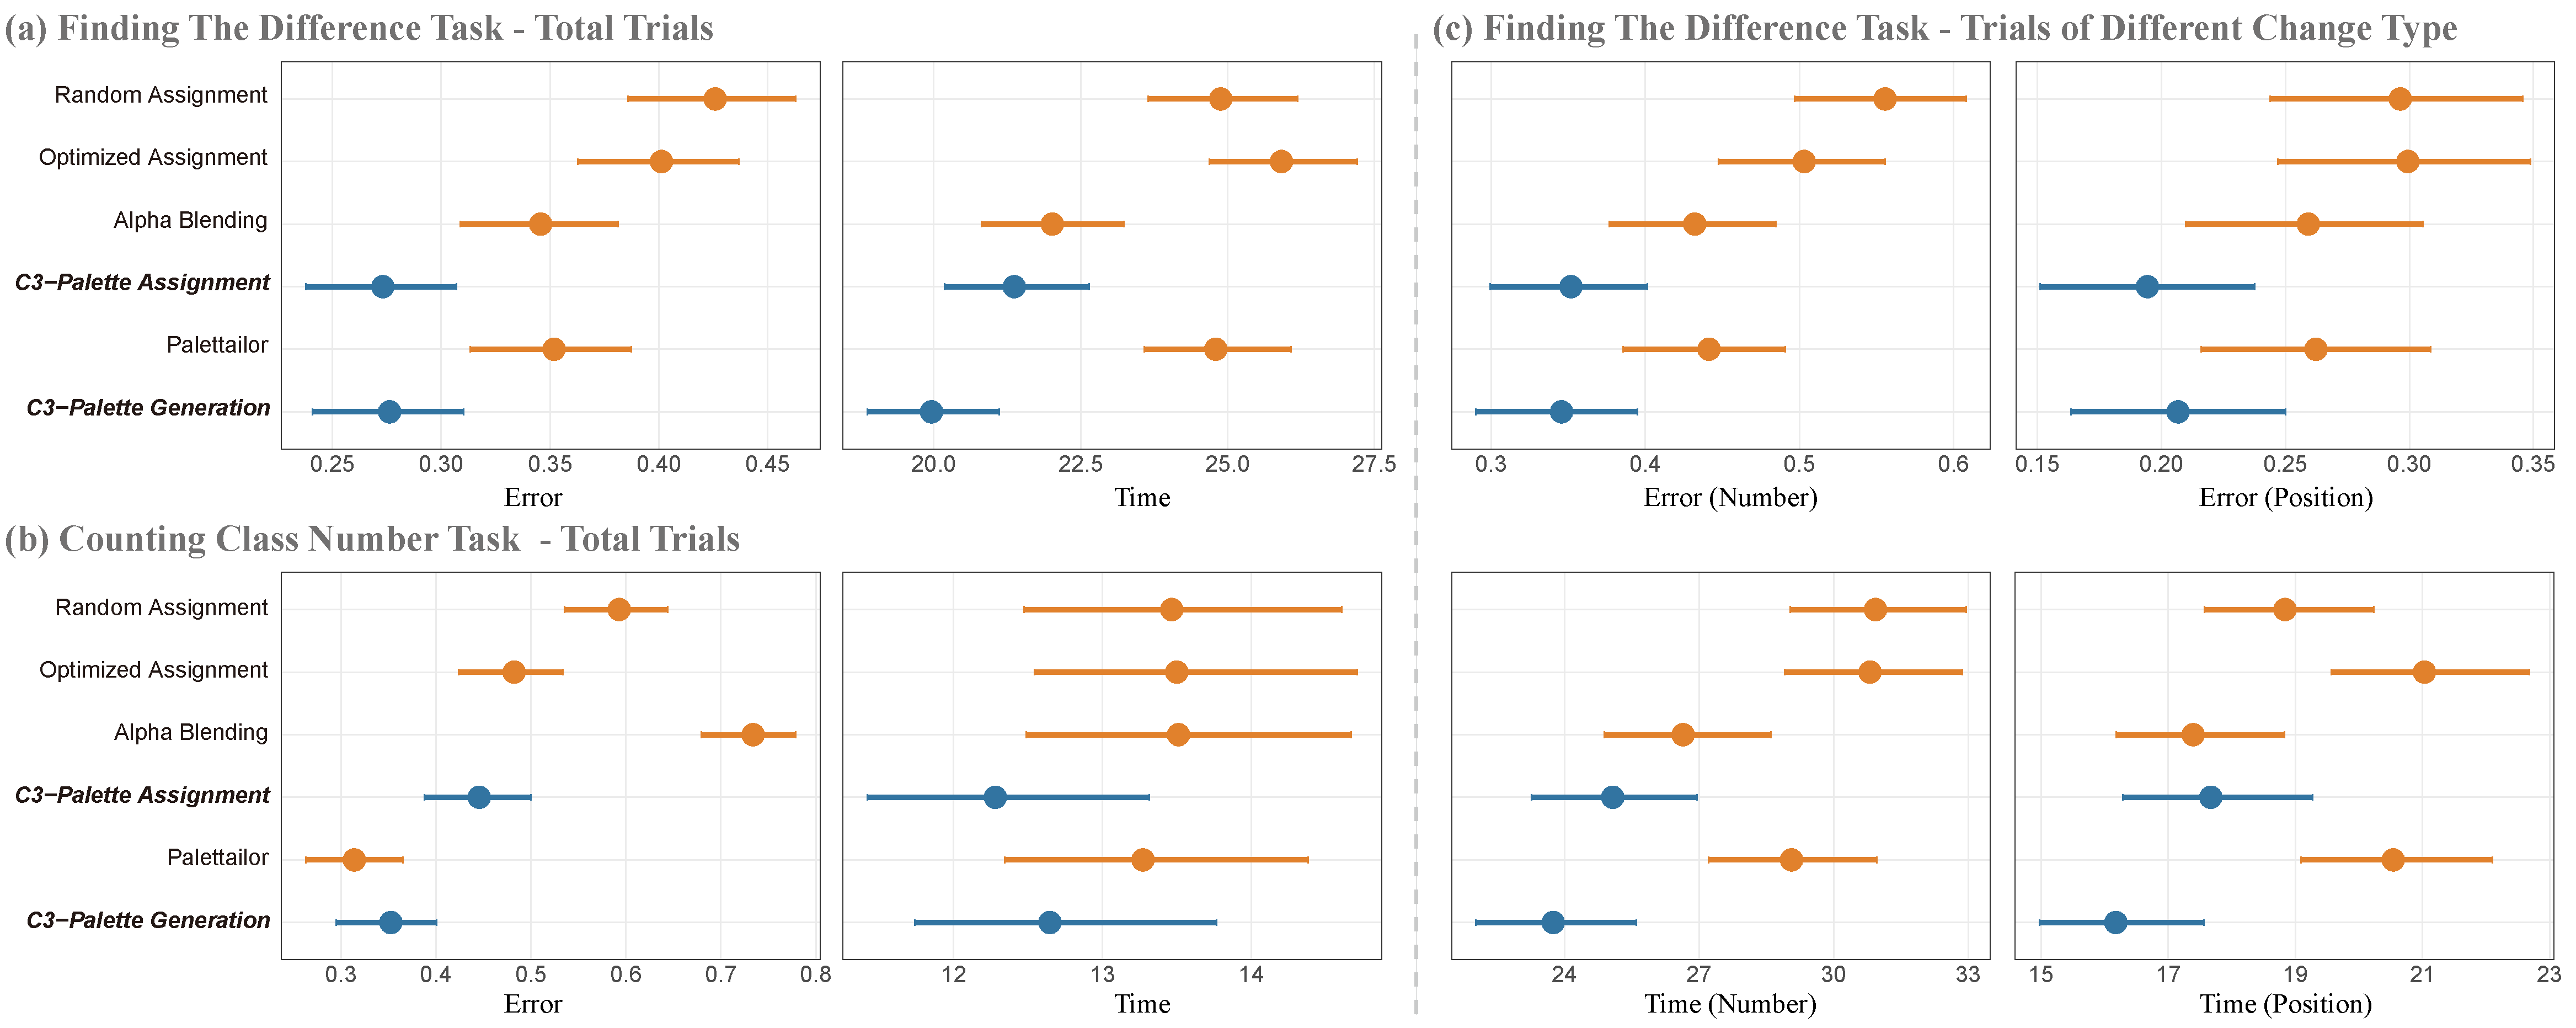
\includegraphics[width=1\linewidth]{figures/user-result-formal.pdf}
\caption{Confidence interval plots and statistical tables for the two online controlled experiments. Error bars represent $95\%$ confidence intervals. Each table shows the statistical test results of C3-Palette Generation condition with other conditions, including the mean with $95\%$ confidence interval ($\mu\sim$95\%CI), the W-value and p-value from the Mann-Whitney test, and the effect size ($d\sim$95\%CI).
}
\vspace*{-3mm}
\label{fig:userResults}
\end{figure*}

\subsubsection{Results}
\
\newline
Following previous studies, we analyzed the results using 95\% confidence intervals, and also conducted Mann-Whitney tests to compare the differences between conditions. The non-parametric test was used due to observations of non-normally distributed data from our pilot study. In addition, we computed the effect size using \emph{Cohen's d}, i.e., the difference in means of the conditions divided by the pooled standard deviation. We used ANOVA to examine the interaction effect between variables.


Results of the online experiment are shown in Fig.\ref{fig:userResults} (a).
First, we found that our approach(\emph{C3-Palette Assignment} and \emph{C3-Palette Generation}) leads to a significantly lower error rate than all benchmark conditions. For consuming time, \emph{C3-Palette Generation} has significantly less time (\emph{$p = 0.003$}) than \emph{Alpha Blending} condition while \emph{C3-Palette Assignment} has no significant difference (\emph{$p = 0.095$}), and our approach has significantly less time than all other benchmark conditions(\emph{$p < 0.001$}). The result indicates that our palette generation method(\emph{C3-Palette Generation}) has a better performance than benchmark conditions in the ``spot-the-difference'' task (\textbf{H1} confirmed). As for color palette with a larger range of brightness and saturation, our approach(\emph{C3-Palette Assignment}) is better than most conditions and is at least comparable to \emph{Alpha Blending} condition(\textbf{H2} confirmed).


%Second, we compared our approach to other conditions based on two different change types(\emph{Point Number Change} and \emph{Point Position Change}).
%For \emph{Point Number Change}, as shown in the top row of  Fig.\ref{fig:userResults} (c), our approach(\emph{C3-Palette Assignment} and \emph{C3-Palette Generation}) leads to a significantly lower error rate than all benchmark conditions, including \emph{Random Assignment} and \emph{Optimized Assignment}(\emph{$p < 0.001$}), \emph{Alpha Blending} and \emph{Palettailor}(\emph{$p < 0.05$}). \emph{C3-Palette Generation} condition has a better performance on consuming time than all other benchmark conditions, while \emph{C3-Palette Assignment} is just comparable to \emph{Alpha Blending} condition.
%For \emph{Point Position Change}, we observed that our approach has significant lower error rate than \emph{Random Assignment} and \emph{Optimized Assignment}(\emph{$p < 0.01$}), while there's no significant difference with \emph{Alpha Blending} and \emph{Palettailor}. \emph{C3-Palette Generation}) leads to a significantly lower consuming time than all benchmark conditions(\emph{$p < 0.001$}) except \emph{Alpha Blending}(\emph{$p = 0.044$})(\textbf{H3} confirmed).
Second, we compared error and time with regard to different change magnitudes, and found that smaller magnitude leads to larger error rate and consuming time (as shown in Fig.\ref{fig:userResultsVar} (a) left). This indicates that there exists an significant interaction effect between \emph{change magnitude} and performance, i.e., \emph{change magnitude} would affect user performance. We did the same test to \emph{change type}, the results show that \emph{point number change} is much more difficult than \emph{point position change}(\textbf{H3} confirmed).


Finally, we did not find significant interaction effect between \emph{colorization methods} and \emph{change magnitude} or \emph{change type}, meaning that the effect of our method is not necessarily influenced by the magnitude of change between the two scatterplots or the different change type of classes (\textbf{H4} not confirmed).

\begin{figure*}[h]
\centering
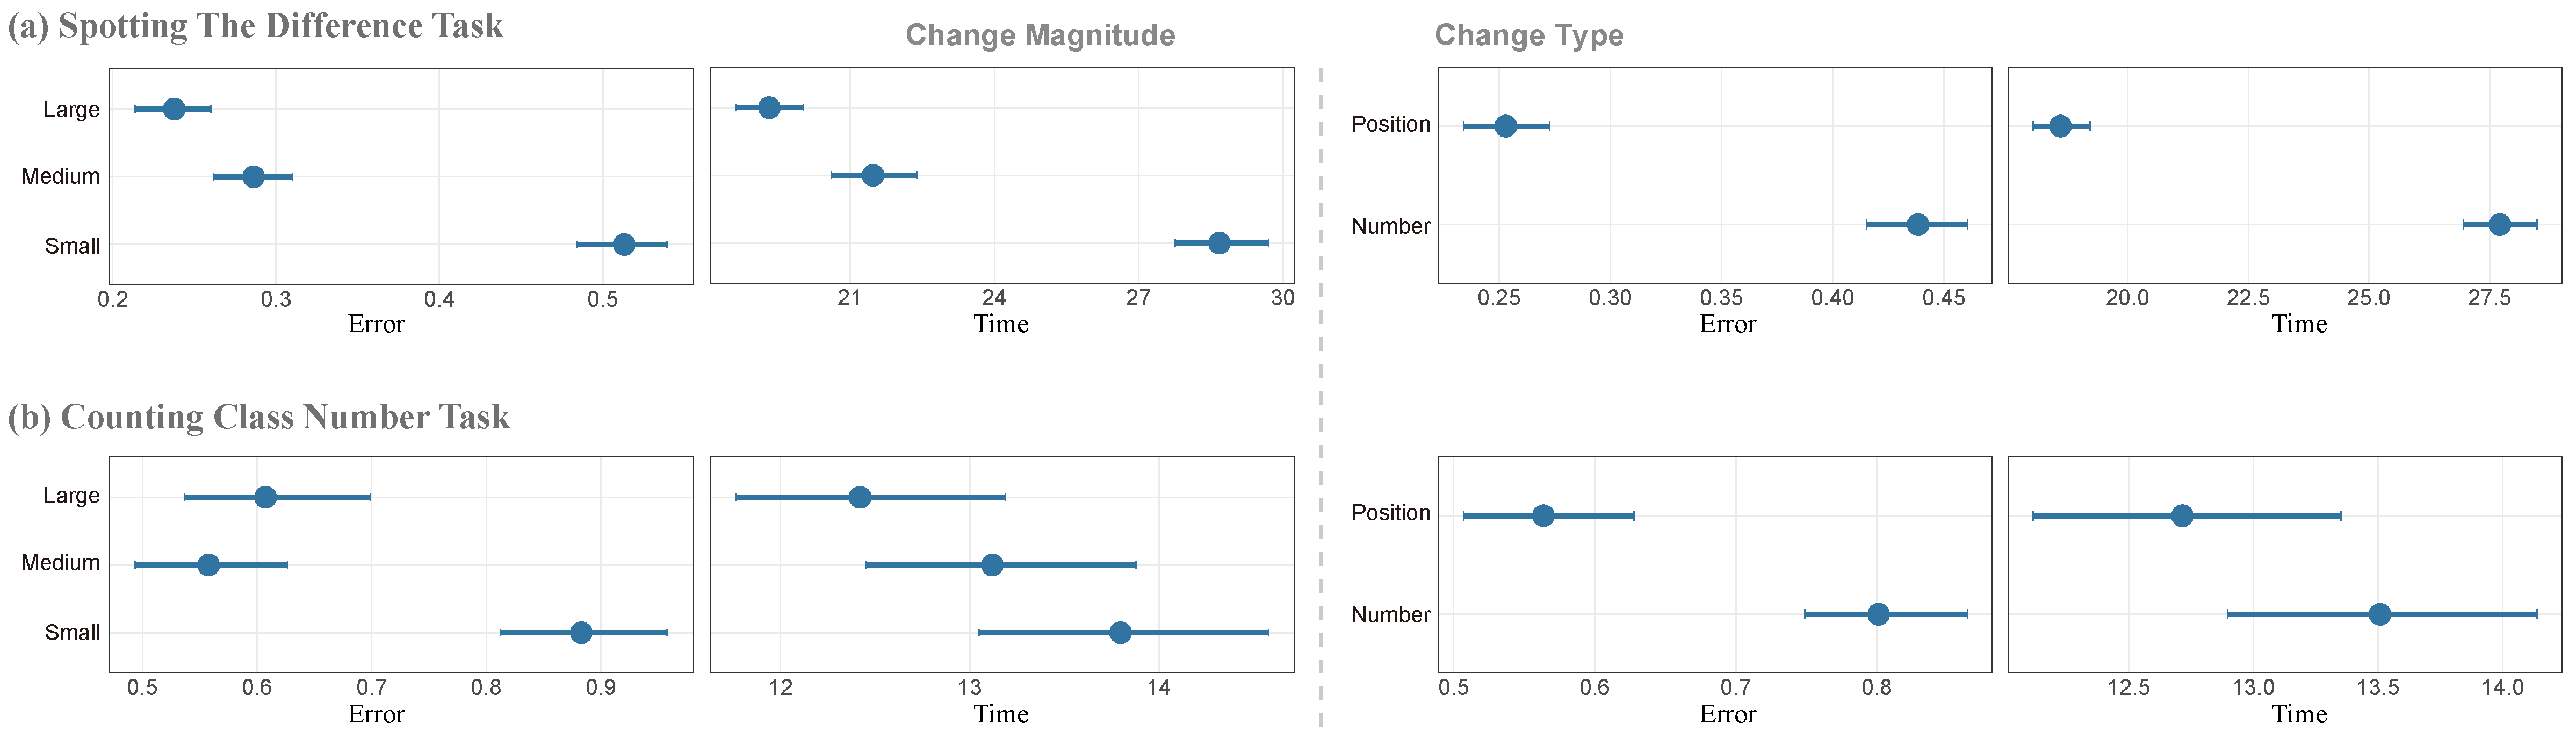
\includegraphics[width=1\linewidth]{figures/user-result-formal-variables.pdf}
\caption{Confidence interval plots for the two online controlled experiments. (left) Plots for \emph{change magnitude} based on error and time; (right) plots for \emph{change type} based on error and time.
}
\vspace*{-3mm}
\label{fig:userResultsVar}
\end{figure*}

\subsection{Experiment 2: Counting Class Number}
\label{subsec:onlinestudy2}
To evaluate whether our approach can fundamentally support the visual separability of the classes in each scatterplot, we conduct an online ``counting class number'' experiment through Amazon Mechanical Turk (AMT) with 81 participants. The experimental design was similar to the first study, but we set up with different task during the experiment.
We expected to see different patterns of the discriminability across different conditions. Specifically, our methods would lead to a shorter error and time than \emph{Random Assignment} and \emph{Alpha Blending} conditions.

\vspace{.3em}
\noindent{\textbf{Hypotheses.}} We hypothesized that our approach would generally be more effective than the benchmark methods on the discrimination tasks, and that this effect would not vary based on \emph{change magnitude} or \emph{change type}.
\begin{itemize}[noitemsep]
\setlength{\itemsep}{5pt}
    \item[\textbf{H1.}] Our color generation method (\emph{C3-Palette Generation}) outperforms the benchmark conditions (\emph{Random Assignment}, \emph{Optimized Assignment}, \emph{Alpha Blending}) and our assignment method(\emph{C3-Palette Assignment}), while is comparable to  \emph{Palettailor} on the task performance.

    \item [\textbf{H2.}] Our color assignment method (\emph{C3-Palette Assignment}) based on \emph{Tableau-20} outperforms the benchmark conditions (\emph{Random Assignment}, \emph{Alpha Blending}), while is comparable to \emph{Optimized Assignment} condition on the task performance.

    \item [\textbf{H3.}] Other independent variables(\emph{change magnitude} and \emph{change type}) would have no effect on discrimination task between different conditions.

    \item [\textbf{H4.}] There would be no interaction effect between colorization methods and other independent variables(\emph{change type} and \emph{change magnitude}).
\end{itemize}
\subsubsection{Experimental Design}
\
\newline
\vspace{.3em}
\noindent{\textbf{Task \& Measures. }}
Following previous methodologies~\cite{Wang2018, Lu21}, each participant was asked to perform a \emph{counting class number} task.  We asked participants to identify how many classes(colors) are there in the given two scatterplots and then choose an answer among several options below the two scatterplots. We recorded the participant's answer and response time for each trial, and counted the \emph{error}  by calculating the differences between the participant's answer and the actual number of classes(each scatterplot has $8$ classes in our experiment). %is $1$ if the participant's response not equal to the actual class number, else $0$.


\vspace{.3em}
\noindent{\textbf{Pilot Study \& Power Analysis.}}
This setting is similar to Experiment 1. We invited $29$ participants to do the pilot study and the results were in further fed into a power analysis. With an effect size Cohen's $d$ of $0.6$, the power analysis suggested a minimum number of $50$ participants for the discriminability task. See the supplementary material for more details.

\vspace{.3em}
\noindent{\textbf{Participants.}}
We finally recruited $52$ participants(as shown in Table.~\ref{tab:participantDetail}) for the experiment on Amazon Mechanical Turk.
According to the completion time in the pilot study, we paid each participant \$$1.5$ for the task based on the US minimum hourly wage.
No participant claimed color vision deficiency on their informed consent.

\subsubsection{Results}
\
\newline
Results of this visual separability experiment are shown in Fig.\ref{fig:userResults} (b).
Through this study we found that first \emph{C3-Palette Generation} is comparable to \emph{Palettailor} while leads to a significantly lower error rate(\emph{$p<=0.001$}) than all other benchmark conditions. Specifically, \emph{C3-Palette Generation} has a significantly lower error rate(\emph{$p=0.002$}) than \emph{C3-Palette Assignment}(\textbf{H1} confirmed).
Second, \emph{C3-Palette Assignment} has higher performance than the benchmark conditions (\emph{Random Assignment}, \emph{Alpha Blending}) and is comparable to \emph{Optimized Assignment}(\textbf{H2} confirmed).
For other independent variables, as shown in Fig.\ref{fig:userResultsVar} (b), we found that there existed a significant difference between \emph{Small change magnitude} and \emph{Medium} and \emph{Large}. \emph{Point position change} has a much lower error rate than \emph{point number change}. And their time has both a tendency to gradually increase. This indicates that \emph{change magnitude} and \emph{change type}) have an effect on discrimination task between different conditions (\textbf{H3} not confirmed). 
Finally, we did not find significant interaction effect between \emph{colorization methods} and \emph{change magnitude} or \emph{change type}, meaning that the effect of different methods for visual discriminability is not 
necessarily influenced by the magnitude of change between the two scatterplots or the different change type of classes (\textbf{H4} confirmed).
\vspace{.3em}
\subsection{Discussion}
In summary, we evaluated the effectiveness of our approach against the benchmark conditions through two online studies. 
We found that first, our methods outperform the benchmark methods on juxtaposed comparison tasks, and their effects are not necessarily influenced by the change magnitude of the two scatterplots or the change type of each class. 
The performance of \emph{Optimized Assignment} is comparable to \emph{Random Assignment}, this is reasonable, since \emph{Optimized Assignment} mainly cares about the visual separability of different classes, thus it might assign the less salient color to the changed class while \emph{Random Assignment} would assign salient color even though the whole separability of the scatterplot is not very good. This also provides an explanation for \emph{Alpha Blending} which is based on the result of \emph{Optimized Assignment}.
Second, our experimental methods (\emph{C3-Palette Generation} and \emph{C3-Palette Assignment}) generally support the fundamental visual separability of the classes. It is worth noting that the error rate of \emph{C3-Palette Generation} is comparable to \emph{Palettailor} which is the start-of-the-art palette generation method for visual discriminability, while \emph{C3-Palette Assignment} is comparable to \emph{Optimized Assignment} which is the start-of-the-art palette assignment method for visual discriminability. This indicates that our approach maintains the class distinction of the scatterplot while enhances the class saliency to help observe changes between different scatterplots.
Third, we found that \emph{change magnitude} and \emph{change type} influence the performance of the \emph{counting class number} task. The potential explanation is that large change between scatterplots will attract participants' attention, thus make it easy to distinct different classes. This is also reasonable for \emph{change type} since point position change is easier to distinguish than point number change.
It's obvious that \emph{Alpha Blending} has a much lower error rate than other methods for discrimination task. As one of the participants said, ``The ones that were harder were ones that had colors that when they overlapped would change color. It made it hard to tell if it was the same color or if it was a new color. When the colors were uniform and all the same opacity, it was much easier.'' \emph{Alpha Blending} condition changes the opacity of unchanged classes to make the unchanged classes more distinct, but this will generate new color by color blending, so as to make it hard to distinct colors.

Some limitations exist in our evaluation.
First, our experiment mainly focuses on error rate and time comsuming, while other measurements are not explored, such as click order of the changed classes and time consuming for each click. These might reflect some interesting results for different \emph{cluster type}.
Second, our experiment focuses on identifying the differences between two scatterplots, which is a simplified situation, since in real-world cases often more than two visualizations are compared.
Third, we cannot further analyze the effect of \emph{change type}, given the current study design, though we did observe some trends that for certain types of change, our methods are more effective.
That brings us to a series of more fundamental questions: how can we properly define the types of changes? What is the just noticeable change magnitude for each change type?
Further research is needed to answer these questions so that our approach can be thoroughly evaluated.
